\documentclass[11pt]{article}
\usepackage[fleqn]{amsmath}
\usepackage{amssymb}
\usepackage{mathrsfs}
\usepackage{graphicx}
\usepackage{float}
\usepackage{subcaption}
\usepackage{relsize}
\usepackage{listings}
\usepackage{tikz}
\usepackage{url}
%\usepackage{breqn}
\lstset{language=Python,
    frame=single,
    breaklines=true,
    postbreak=\raisebox{0ex}[0ex][0ex]{\ensuremath{\color{red}\hookrightarrow\space}}
}
%%\usepackage[margin=2cm]{geometry}
%%\floatstyle{boxed}
\restylefloat{figure}
\newcommand{\Prop}{\textbf{Proposition: }}
\newcommand{\Prob}{\textbf{Problem: }}
\newcommand{\Prf}{\textbf{Proof: }}
\newcommand{\Sol}{\textbf{Solution: }}
\newcommand{\Nats}{\mathbb{N}}
\newcommand{\Ints}{\mathbb{Z}}
\newcommand{\Rats}{\mathbb{Q}}
\newcommand{\Reals}{\mathbb{R}}
\newcommand{\Comps}{\mathbb{C}}
\newcommand{\Prb}[1]{P\left( #1 \right)}
\newcommand{\PT}[1]{P\left( \text{#1} \right)}
\newcommand{\PCon}[2]{P\left( #1 \mid #2 \right)}
\newcommand{\PConT}[2]{P\left( \text{#1} \mid \text{#2} \right)}
\DeclareMathOperator{\E}{\mathbb{E}}
\DeclareMathOperator{\tr}{\textbf{tr}}
\newcommand{\thus}{\quad\mathlarger{\mathlarger{\mathlarger{\Rightarrow}}}\quad} 
\usepackage[left=2cm,right=2cm,top=2cm,bottom=2cm,nohead]{geometry}
%%\newcommand\scalemath[2]{\scalebox{#1}{\mbox{\ensuremath{\displaystyle #2}}}}
\begin{document} 
\setcounter{secnumdepth}{1}
\title{229 Project Milestone: Generating Ad Hoc Curricula}
\author{Andrew Lampinen (lampinen@stanford.edu)}
\date{}
\maketitle

\section{Introduction}
Often in machine learning, proofs of convergence of learning algorithms assume that the data distribtuion is static over the course of learning. However, work on Curriculum Learning \cite{Bengio2009} has shown that in practice, altering the data distribution over the course of learning can improve results, at least in some cases. Specifically, starting with easier examples first and then progressing to harder examples can be beneficial, possibly even making a task learnable when it is not learnable from a reasonable amount of data using the standard strategy. This idea has proven useful in many contemporary networks, e.g. \cite{Graves2016}.\par
However, in many cases we lack explicit knowledge about the structure of the problem from which we could construct a curriculum. For example, on the MNIST task, how do we decide which examples are ``easy'' or ``hard?'' Perhaps we could have human coders evaluate every image and call an image harder the more they disagree, but that would be prohibitively expensive. Is there a way we can craft curricula for a task while remaining more agnostic to what the task actually is (ideally just from the data vectors and labels)?
\section{Proposed ad-hoc curricula}
\subsection{Data recombination and central tendencies}
First, we consider a way of crafting curricula which, while not entirely data agnostic, we think may be beneficial in a wide variety of practical scenarios. The basic idea is very simple. If our data are noisy samples from some distribution, we might think that by combining/averaging data points with the same labels, we will generally yield less noisy/better estimates of the central tendency of the data distribution for this class, which may provide a better place to begin learning. In an ideal case where the data form distinct clusters, the centroids of the clusters will be far from eachother even if individual exemplars may lie close to other clusters. Thus the averaged examples may be ``easier'' in the sense Bengio et al. described. For example, on MNIST the average of all the 0 examples is probably more 0 like than many of the individual examples. Thus, averaged data may provide ``easier'' examples. However, this intuition requires making a few important assumptions about the distribution of the data for each class:
\begin{enumerate}
\item The data are well represented by their central tendency. (E.g. in an XOR problem, the mean of either class would be a poor representation of that class, because the means of the classes coincide.) 
\item The variance within the class is not large relative to the between-class variance. (The central tendency has to convey useful information.) 
\end{enumerate}
For example, on a visual recognition task like ImageNet these assumptions would likely be violated -- the average of all dog images in ImageNet would likely just be a muddy blur, which would look nothing like a dog. Furthermore, the variance in pictures of dogs is very high, the dog could be facing the camera, jumping after a frisbee, etc. Thus creating curricula by averaging might not be as helpful. However, even here there might be useful color information, for instance, which could be obtained from the average. Similarly, if there is a large contingent of images that center the face of the dog, there might be useful information in the average about dog faces. We think it is an open question whether this strategy would be beneficial there. \par
\subsection{Confusing examples from previous training}
We also considered the possibility of deriving an ad-hoc curriculum by training a classifier with no curriculum, and then ranking example easiness by what examples it found most confusing (e.g. easy examples have large positive margin, hard examples have small positive to large negative margin). This can be seen as an approximation to one of the original curricula suggested by Bengio and colleagues, where instead of using the unknown true margin as a measure of easiness we are using the margin from our approximation to the true classification boundary. \par
This bears some resemblance to active learning strategies that have been suggested previously \cite[e.g.]{Krogh1995}. However, it is distinct because we are deriving a curriculum rather than choosing examples actively online. Furthermore, most active learning methods have favored selecting hard examples at all times, here we are favoring putting them off until after easy examples have been seen. 
\section{Preliminary test}
First, we tested our strategies on the toy example used in \cite{Bengio2009}. The task is simply to learn a linear classifier with a single layer neural network (i.e. there is no bias, the true target function lies within the space of single layer neural networks). One curriculum they suggested was sorting the data by the margin, with the idea that points farther from the classification boundary are ``easier,'' in the sense that the classifier boundary can be more inaccurate and still classify them correctly. Bengio and colleagues found this resulted in better generalization after training on 200 examples. \par
We used both this curriculum strategy and a no-curriculum random-order training strategy for comparison. To test our ideas we created: 
\begin{itemize}
\item a data recombination ad-hoc curriculum consisting of 200 examples ordered as follows:
    \begin{enumerate}
    \item 10 positive and 10 negative examples (alternated), each created by averaging 10 examples of the expected class
    \item 10 positive and 10 negative examples (alternated), each created by averaging 5 examples of the expected class
    \item The remaining 160 examples were the last 160 examples the non-curriculum network saw. 
    \end{enumerate}
\item a previous classifier-based ad-hoc curriculum consisting of 200 examples sorted by a previous classifier's margin on them after training was complete (from largest to smallest margin). 
\end{itemize}
We evaluated these strategies on two metrics:
\begin{itemize}
\item Error on 1000 new test examples
\item Dot product of learned parameters with true parameters (normalized by the lengths of the vectors)
\end{itemize}
See Figure \ref{toy_errors} for the density plot of the final test error across 100 runs, and Figure \ref{toy_dots} for the evolution of the weights over time averaged across 100 runs. The non-curriculum network achieved an average generalization error of 28.7\% with a standard deviation of 3.7\%, and an average cosine distance from the true weights of 0.363. Bengio and colleagues' margin-based curriculum achieved an average generalization error of 26.0\% with a standard deviation of 4.3\%, and an average cosine distance from the true weights of 0.295. 
\begin{figure}
\centering
\begin{subfigure}{0.38\textwidth}
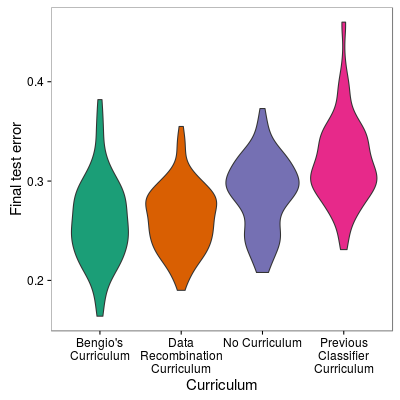
\includegraphics[width=\textwidth]{toy_results/violin_plot.png}
\caption{Final error rates by curriculum (density over 100 runs)}
\label{toy_errors}
\end{subfigure}
~
\begin{subfigure}{0.57\textwidth}
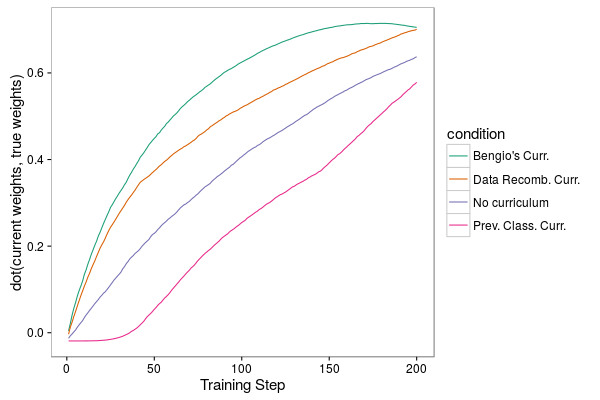
\includegraphics[width=\textwidth]{toy_results/dot_trace_plot.png}
\caption{Evolution of dot product between true parameters and current parameters over learning (averaged over 100 runs)}
\label{toy_dots}
\end{subfigure}
\caption{Results on toy model from \cite{Bengio2009}}
\label{preliminary_results}
\end{figure}
\subsection{Data recombination results}
The data recombination curriculum performed nearly as well on average as the curriculum used by Bengio et al., and performed slightly more consistently. It achieved a mean generalization error of 26.3\% with a standard deviation of 3.3\%, which was significantly better than the non-curriculum strategy (paired $t$-test, t(99) = 7.9, p = 3.2e-12), and not significantly different than Bengio's curriculum (paired $t$-test, t(99) = -1.0, p = 0.32). It achieved an average cosine distance from the true weights of 0.299.\par
This is a very promising result, we were able to craft a curriculum without using knowledge about the data that performed as well as the curriculum used by Bengio and colleagues which relied on explicit information about the structure of the task.
\subsection{Previous classifier curriculum results}
By contrast, the previous classifier curriculum performed quite poorly, in fact worse than the non-curriculum. It achieved a mean generalization error of 31.9\% with a standard deviation of 4.2\%, which was significantly worse than the non-curriculum strategy (paired $t$-test, t(99) = -8.8, p = 5.3e-16), and an average cosine distance from the true weights of 0.422.\par
It is possible that these results were so poor because the margin estimates are not just wrong, they are wrong in a biased way, since they are all computed from the same classifier. Using many previous classifiers and averaging margins across them might provide more robust estimates that would allow this strategy to work. However, on complex problems like MNIST where training each classifier takes a non-trivial amount of time, this would become prohibitively expensive (at least with the computational resources we have access to). Thus we will not pursue this strategy further in this project.
\section{Future Directions}
\subsection{MNIST \& Noisy MNIST}
Now that we have demonstrated the benefits of the data recombination strategy for the toy task, we hope to validate it on a more complex task. Specifically, we will try it on the MNIST digit recognition task, using a simple convolutional neural network. However, the MNIST task has been thoroughly explored, and it may be difficult to achieve better performance there. Thus we will also consider a noisy version of the MNIST data where we add (a very large amount of) independent noise to each training image. This is a setting where data averaging may be very helpful (and in many real-world classification tasks our data may be much noisier than the relatively clean MNISt dataset). 
%\subsection{Better curricula}
%Consider clustering and finding several central tendencies for each class instead of just one, e.g.


\bibliographystyle{acm}
\bibliography{cs229_project_citations}
\end{document}
